\section{Introduction}
\label{sec:introduction}

The proliferation of cloud services is changing the way we think about
wide-area application design.  Developers today do not need to build storage
or authentication mechanisms from scratch, but may instead synthesize them by
combining existing cloud-hosted services.  While this reduces up-front
development costs, it is not sustainable in the long run,
since these services regularly fail, adopt incompatible trust models, and
unilaterally introduce breaking changes without warning.  This paper
presents Syndicate, a system that synthesizes custom stable storage
from unstable services by implementing a programmable ``storage kernel'' that spans
wide-area networks.

Reusing existing software to create new software is generally good engineering practice.
However, maintaining an application that relies on chronically unstable services
creates a standing operational cost, which has proven onerous enough in practice that
many developers end up building their own equivalent services internally in the
long run.  This has already happened with popular applications
like Facebook, Snapchat, and Uber, for example.

This outcome has both negative technical and social consequences.  On the
technical side, it duplicates code and bugs, and requires each application to
implement its own storage ``drivers'', access controls, user authentication,
identity management, and data discovery and indexing logic.  Even then, a single
broken service can render many applications unavailable, and require each one
to be independently patched.

On the social side, this outcome harms both developers and users.  Because the
application implements all of the data proccessing and access logic, a user can
only interact with their data if the application is available and permits it.  This puts users at
the mercy of developers, and makes developers liable for securely mediating all access
to all user data.
%developers? maybe you mean service providers?

The rise of two new technologies enables a solution to these problems.  First, the
ubiquitous availability of \textit{cheap personal cloud storage} gives
applications a way to store user state on user-controlled storage while keeping
it available.  Users would no longer need to exclusively rely on the application to access their data,
and developers would no longer need to be responsible for hosting it.

Second, the rise of \textit{self-sovereign identity systems} like
Blockstack~\cite{blockstack} and Keybase~\cite{keybase} allow users to
securely advertise their \textit{current} identity tokens, like public keys, in a
non-repudiable way.  Crucially, self-sovereign identity systems do not
require trust in 3rd parties (unlike conventional identity providers)
and do not require users to directly manage public keys (unlike PGP).
Such systems are currently backed by the security of a popular proof-of-work blockchain, like
Bitcoin's blockchain~\cite{bitcoin}, where anyone can append a new record
but no single principal possesses the computational power required to remove it.

\begin{figure}[h!]
\centering
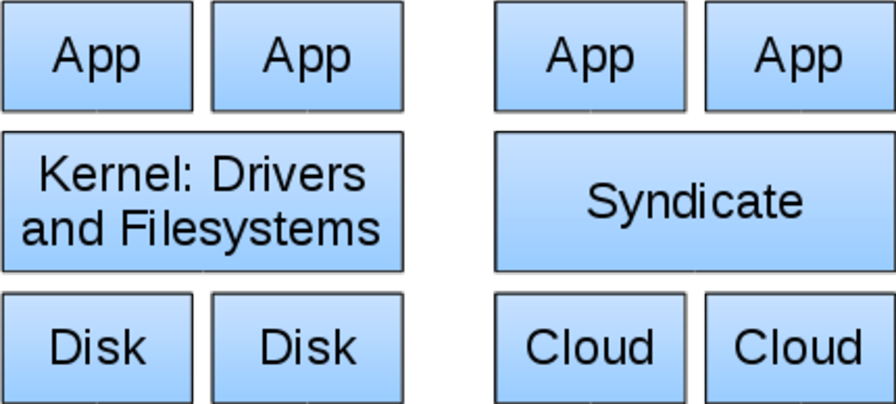
\includegraphics[width=0.5\textwidth]{figures/kernel}
\caption{\it As a storage kernel, Syndicate fulfills the same role for wide-area
applications and underlying storage and identity services as an OS kernel does
   for userspace programs, storage hardware, and access control frameworks.}
\label{fig:kernel}
\end{figure}

The goal of this work is to enable the creation of applications that can
leverage its users' personal cloud storage for hosting user-specific state, and
rely on a self-sovereign identity system to enable users to authenticate one
another, authenticate shared data, and authenticate themselves to the application.
Such applications would not have the aforementioned problems, since they
treat users as the authoritative sources of both identity and data.  In cases
where no cross-user indexing is required, applications would no longer need
servers:  the developer simply serves the client directly to users via his/her
personal cloud storage, and users authenticate it with the shared self-sovereign
identity system.

However, implementing these applications is difficult today,
because there does not exist a ``storage kernel'' to connect them to
self-sovereign identity and storage implementations (Figure~\ref{fig:kernel}).
Applications that use multiple services today nevertheless each implement and
kernel-like functionality internally (Section~\ref{sec:motivation}), which motivates us to
explore designing the storage kernel up front.

State-of-the-art systems like Blockstack~\cite{blockstack},
libcloud~\cite{libcloud}, and Infinit~\cite{infinite} come close to this
end by implementing a service ``driver'' layer to
store data across multiple storage providers.  However, this is not
sufficient to implement applications with non-trivial storage requirements,
because several key challenges remain:

\textbf{Storage is data-dependent}. Storage spans multiple
administrative domains, but deciding which domain may store data and how it may
do so both depends on the data itself. For example, financial records must leave
an audit trail, and medical records in the US must conform to HIPPA.

\textbf{Data is user-centric}. Users own their data, not applications.
As such, users need end-to-end programmatic control over how their data
can be made available, independently of both applications and services.

\textbf{Storage is asynchronous}. Some storage features require an external
actor to implement correctly, such as migrating cold data to long-term storage
and deleting data after a maximum retention period.

\textbf{The TCB is partitioned by user}.  Users only trust code that runs on their own
devices.  As such, a wide-area kernel cannot be universally trusted.

Our key insight to overcoming these challenges is that a storage kernel
must \textit{additionally} enable user-level control over data-plane operations.
In particular, users must be able to programmatically
control how I/O flows (reads and writes) affect their data.  They must be able to change the
logic that governs I/O flows at runtime, and the logic must be able to
act independently of the user and application.  This is why a driver layer alone is
not enough--driver logic only runs synchronously with I/O, and cannot take
actions on its own.

\begin{figure}[t!]
\centering
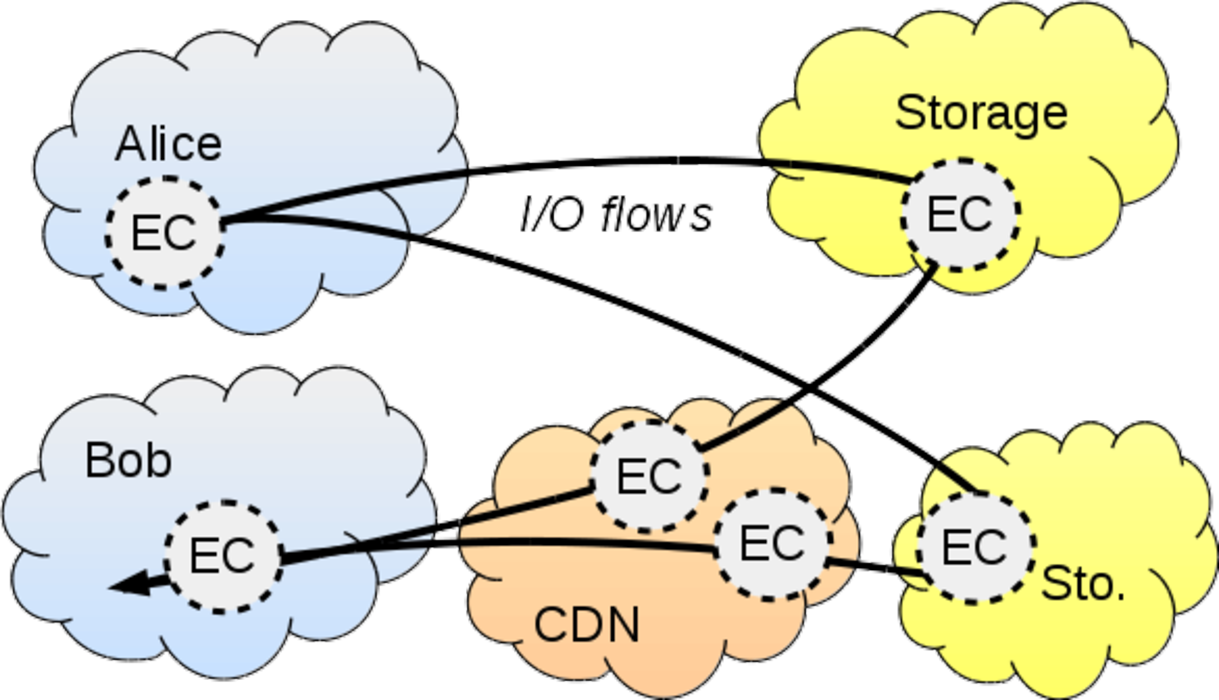
\includegraphics[width=0.5\textwidth]{figures/execution-contexts}
\caption{\it...}
\label{fig:execution-contexts}
\end{figure}

Constructing a user-programmable wide-area kernel is difficult, because the kernel cannot be
universally trusted.  To overcome this challenge, we partition the kernel into a
set of user-owned \textit{execution contexts}
(Figure~\ref{fig:execution-contexts}).  An execution context is a
kernel shard that runs a user-supplied \textit{storage program} to processes I/O
flows on its owner's data.  The task of the storage kernel, then is to 
route I/O flows across the wide-area 
through a dynamic set of storage programs
while achieving end-to-end authenticity and correct flow-processing in the face
of system and service churn.

Syndicate is our prototype wide-area storage kernel.  It provides 
users with one or more horizontally-scalable execution contexts, called
\textit{gateways}, that implement a user-defined data-plane while ensuring
end-to-end authenticity and correctness in the face of system churn and service
misbehavior.  Its key novelty is a control-plane protocol
that leverages a self-sovereign identity system to enable gateways to coordinate in
the presence of untrusted networks and services.  By doing so, Syndicate allows
storage programs to compose in a UNIX-like pipeline across the wide-area,
enabling users to synthesize complex storage features from simple
orthogonal storage programs on top of one or more storage providers.

This paper is organized as follows.  In Section~\ref{sec:related-work}, we
provide more background on blockchains and other state-of-the-art kernel-like systems upon
which we build.  In Section~\ref{sec:motivation}, we characterize two
application domains--scientific storage and SaaS--in which users would
significantly benefit from having a programmable storage kernel.  We present the
design of Syndicate in Section~\ref{sec:design}, its implementation in
Section~\ref{sec:implementation}, and its evaluation in
Section~\ref{sec:evaluation}.  We conclude in Section~\ref{sec:conclusion}.
